% Jamie Nagle's toy jet exercises, reproduced with OT flow matching
% (FLOW_NOTES.md, "Jamie's toy exercises with OT flow matching"). Numbers:
% docs/flow/jamie_otfm/*/*.csv (jamie_report.py) via tables/*.tex
% (jamie_slides_tables.py); figures docs/flow/jamie_otfm/*/*.png (jamie_figs.py).
% Build: cd docs/flow/jamie_otfm/slides && ~/pyext/tectonic_env/bin/tectonic jamie_otfm.tex
\documentclass[aspectratio=169,10pt]{beamer}
\usetheme{default}
\setbeamertemplate{navigation symbols}{}

\usepackage{booktabs}
\usepackage{graphicx}
\usepackage{xcolor}
\usepackage{amsmath}
\graphicspath{{../}{../ex1/}{../ex2/}{../ex3/}{../ex3g/}{../ex4/}{../prior_data/}}

\definecolor{ink}{HTML}{0B0B0B}
\definecolor{ink2}{HTML}{52514E}
\definecolor{muted}{HTML}{898781}
\definecolor{rule}{HTML}{E1E0D9}
\definecolor{wash}{HTML}{F4F3EF}
\definecolor{cUP}{HTML}{EB6834}
\definecolor{cSP}{HTML}{2A78D6}
\definecolor{cHY}{HTML}{1BAF7A}
\definecolor{cTP}{HTML}{4A3AA7}

\setbeamercolor{normal text}{fg=ink}
\setbeamercolor{frametitle}{fg=ink}
\setbeamercolor{itemize item}{fg=muted}
\setbeamercolor{itemize subitem}{fg=muted}
\setbeamerfont{frametitle}{size=\large,series=\bfseries}
\setbeamertemplate{itemize items}{\raisebox{0.15em}{\scalebox{0.6}{$\blacksquare$}}}
\setbeamertemplate{itemize subitem}{--}
\setbeamersize{text margin left=1.1em,text margin right=1.1em}
\setbeamertemplate{frametitle}{\vspace{0.45em}\insertframetitle\par\vspace{-0.25em}%
  {\color{rule}\rule{\textwidth}{0.6pt}}}
\setbeamertemplate{footline}{\hspace{1.1em}{\tiny\color{muted}Jamie Nagle's toy exercises with OT
  flow matching. TOY MODEL: reimplemented toy jets, UE and quenching, not PYTHIA, HIJING or JEWEL}%
  \hfill{\tiny\color{muted}\insertframenumber}\hspace{1.1em}\vspace{0.6em}}

\title{Jamie Nagle's toy exercises with OT flow matching}
\subtitle{Does flow matching keep the jet, its medium-induced radiation and the event's own UE?}
\date{2026-10-06}
% supervision labels, on every result
\newcommand{\suplab}[2]{{\setlength{\fboxsep}{1.2pt}\colorbox{#1!14}{\scriptsize\color{#1!80!black}\textbf{#2}}}}
\newcommand{\UP}{\suplab{cUP}{pure unpaired}}
\newcommand{\SP}{\suplab{cSP}{synthetic paired}}
\newcommand{\HY}{\suplab{cHY}{hybrid}}
\newcommand{\TP}{\suplab{cTP}{true-paired control}}
\newcommand{\snote}[1]{{\scriptsize\color{ink2}#1\par}}
% the same labels as short table tags
\newcommand{\stag}[2]{{\setlength{\fboxsep}{0.8pt}\colorbox{#1!14}{\tiny\color{#1!80!black}#2}}}
\newcommand{\sUP}{\stag{cUP}{pure unpaired}}
\newcommand{\sSP}{\stag{cSP}{synthetic paired}}
\newcommand{\sHY}{\stag{cHY}{hybrid}}
\newcommand{\sTP}{\stag{cTP}{true-paired control}}
\newcommand{\sST}{{\tiny\color{muted}standard}}
% a generated table one size smaller
\newcommand{\tinytab}[1]{{\let\scriptsize\tiny\input{#1}}}
% a generated table scaled to a width
\newcommand{\fittab}[2]{\resizebox{#1}{!}{\input{#2}}}

\begin{document}

% ---------------------------------------------------------------- 1
{\setbeamertemplate{footline}{}
\begin{frame}
\vspace{1.2em}
{\Large\bfseries Jamie Nagle's toy exercises with OT flow matching\par}
\vspace{0.3em}
{\normalsize\color{ink2} Does flow matching keep the jet, its medium-induced radiation and the event's
own underlying event? Four exercises on a toy whose truth is known\par}
\vspace{0.9em}
\small
\begin{itemize}\setlength\itemsep{0.25em}
\item \textbf{Subtraction:} no halo, but the solved flow gives 25\% of the jet core to the background, and
  on quenched jets 71-82\% of the recoil. No loss change fixes it: the network's one-step estimate is
  right; the transport is not
\item \textbf{Translation:} a deterministic flow keeps each jet and under-quenches; the noise-driven model
  gets the quenched population, not the jet-by-jet randomness, unless trained on true pairs
\item \textbf{With the UE:} the matching cost decides. With a near/far cost the flow keeps this event's UE
  as exactly as the truth and recovers 114\% / 80\% of the core / ring change
\item \textbf{Prior against data:} the data change the answer measurably, but the prior still decides
  most of it
\end{itemize}
\vspace{0.6em}
\scriptsize
\textbf{Every result is labelled by its supervision:}\quad \UP{} independent pools, paired by the OT
plan\quad \SP{} mixtures built from the prior and UE pools, trained to their own UE\quad \HY{} both\quad
\TP{} trained on true pairs (a positive control)
\vfill
{\footnotesize\color{muted} TOY MODEL: a reimplementation of the deck's toycalo listings, not PYTHIA,
HIJING or JEWEL. Seed 0 unless stated; 20k held-out events per test; 32 A6000 GPU hours of training. Full
log \texttt{FLOW\_NOTES.md}, results \texttt{docs/flow/jamie\_otfm}\par}
\end{frame}}

% ---------------------------------------------------------------- 2
\begin{frame}{Setup}
\begin{columns}[T]
\column{0.5\textwidth}
\scriptsize
\textbf{The toy} (reimplemented from Jamie's listings; his code was not available)
\begin{itemize}\setlength\itemsep{0.1em}
\item $24 \times 64$ towers, $|\eta| < 1.1$, periodic $\varphi$; jets $E^{-4}$ in 20-80 GeV, one or two
  prongs; UE: gamma towers (mean 0.6 GeV, $v_2$) plus minijets
\item quenching: $f \sim$ Beta(2,6); particles lose $(1-f)$ and spread by $(1+f)$; $fE$ goes into
  $\approx 15$ recoil particles at $0.3 < r < 1.0$. Each draw is random: one vacuum jet, many quenched
  versions
\item checks against Jamie's numbers: cone 28.4 $\to$ 22.0 GeV (28.2 $\to$ 21.9), ring 0.4 $\to$ 6.6
  (0.4 $\to$ 6.6), $\rho A$ offset/RMS +0.85/4.5 GeV (+0.7/4.4), UE-only fakes 88\% (88\%)
\item separate parents for every pool (40k each) and test set (20k); the hidden truth only scores
\end{itemize}
\textbf{Regions} around the jet axis: core $R < 0.4$, recoil ring $0.4$-$1.0$, far $R > 1.0$ (towers
there change in 22\% of quenched jets: the protected region is not exactly untouched)
\column{0.48\textwidth}
\scriptsize
\textbf{The models} (the UVCGAN-S ViT network, 32M; log-energy coordinates; batch 256)
\begin{itemize}\setlength\itemsep{0.1em}
\item \textbf{D}: deterministic OT-CFM. A source image flows to its OT-matched target; one output per
  input
\item \textbf{C}: conditional FM on the OT pseudo-joint. The input is a fixed second channel; noise flows
  to the matched target; one image per noise draw
\item \textbf{the OT plan} (exact, squared distance of whole images) matches the UE in subtraction and
  Exercise 4 and the position in Exercise 3, hardly the jet's energy (an audit before training). Exercise 4
  also runs the pre-specified near/far cost
\item 1.5 GPU-hours per baseline; continuations 4000 updates from it with one change; extra-term weights
  from a gradient-scale audit, frozen
\item the ODE: midpoint, NFE doubled on validation until stable, frozen before testing
\end{itemize}
\end{columns}
\end{frame}

% ---------------------------------------------------------------- 3
\begin{frame}{Exercise 1: subtraction. The core goes into the background; no halo}
\begin{center}
\fittab{0.92\textwidth}{tables/ex1.tex}
\end{center}
\vspace{-0.2em}
\snote{20k held-out mixtures (jets 20-80 GeV in UE), true axis, $\hat J = M - \hat B$ raw and signed.
Hard-tower loss: $\hat J - J$ on true towers above 1 GeV. Halo: positive $\hat J$ on truth-empty towers in
the cone. Fakes: UE-only events. Continuations: 4000 updates from E1-P, one change each.}
\vspace{0.3em}
\scriptsize
\begin{columns}[T]
\column{0.5\textwidth}
\begin{itemize}\setlength\itemsep{0.15em}
\item \textbf{Jamie's core loss is reproduced, his halo is not} (pre-registered: loss above 10\%, halo
  above 3 GeV), \UP{} and \SP{} alike
\item resolution 2.5 GeV against $\rho A$'s 4.5 (Jamie's fixed network: 2.4-2.6); fakes 0.1\%
\item the offset grows with energy ($-$4.6 GeV at 10-20, $-$8.8 at 50-80 for E1-U)
\end{itemize}
\column{0.48\textwidth}
\begin{itemize}\setlength\itemsep{0.15em}
\item \textbf{what the loss changes:} GeV and balanced masks remove the negative towers (2.7\% $\to$
  0.2\%), trim the halo (2.2 $\to$ 2.0 GeV); ring sums add nothing; the flat prior flattens the energy
  dependence
\item \textbf{what it does not:} the core loss ($-$23 to $-$25\%) and the offset
\end{itemize}
\end{columns}
\end{frame}

% ---------------------------------------------------------------- 4
\begin{frame}{Exercise 1: why the core is lost}
\begin{columns}[T]
\column{0.5\textwidth}
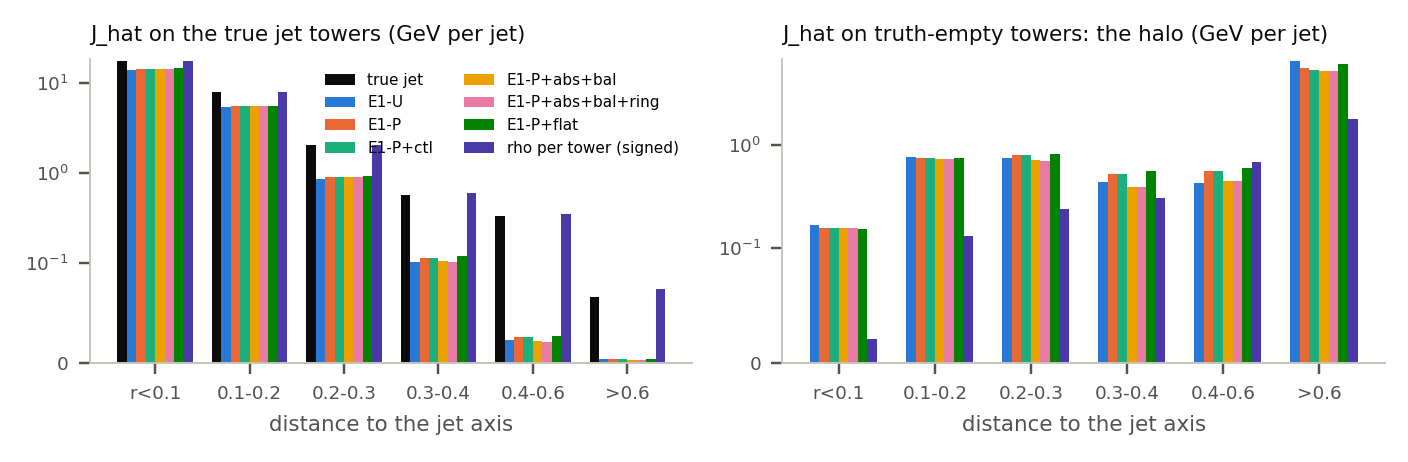
\includegraphics[width=\textwidth]{ex1_rings.png}
\vspace{0.3em}
\fittab{\linewidth}{tables/onestep.tex}
\vspace{0.2em}
\snote{One-step mean: $x_0 + v(0, x_0)$, the regression's estimate of the mean background given the
mixture; solved: the ODE output that is scored. 500 validation mixtures.}
\column{0.48\textwidth}
\scriptsize
\begin{itemize}\setlength\itemsep{0.3em}
\item ring by ring (Jamie's table): the true jet towers keep 14.2-14.4 of 17.7 GeV at $r < 0.1$ and
  lose most of their soft edge; empty towers get under 1 GeV per ring within $R < 0.6$ (4-6 GeV spread
  over the far towers)
\item \textbf{the network's one-step estimate has the core right} (hard-tower error $-$2\%, +1\%;
  $\hat B$ 0.5-0.7 GeV on hard towers, true UE 0.58) and shows Jamie's halo instead (UE fluctuations
  left in the jet: cone offset +1.7, +7.3 GeV)
\item \textbf{the solved flow loses 25\%}: $\hat B$ is 2.0 GeV on the hard towers. The flow carries the
  mixtures onto realistic UE images, and puts the UE's largest fluctuations where the mixture is
  brightest: under the jet core
\item so losses on the one-step surrogate (Jamie's three-part fix, as specified) cannot reach it: their
  terms barely fall in training (abs 0.233 $\to$ 0.216)
\end{itemize}
\end{columns}
\end{frame}

% ---------------------------------------------------------------- 5
\begin{frame}{Exercise 2: a frozen vacuum subtractor on quenched jets}
\begin{center}
\scriptsize
\setlength{\tabcolsep}{3pt}
\begin{tabular}{llrrrrrrr}
\toprule
 & & cone $E$ & girth & ring 0.4-1 & mass & quenched & recoil & ring of \\
 & & shift & shift & shift & shift & jets lost & in $\hat B$ & vacuum jets \\
\midrule
truth &  & -6.27 GeV & +0.027 & +6.09 GeV & -0.005 GeV & 0 & -- & 0.40 GeV \\
\midrule
E1-U & \sUP & 102\% & 85\% & 29\% & -0.40 GeV & 14\% & 4.35 & 1.50 \\
E1-P & \sSP & 108\% & 84\% & 18\% & -0.48 GeV & 15\% & 5.01 & 1.65 \\
E1-P+ctl & \sSP & 110\% & 84\% & 16\% & -0.50 GeV & 16\% & 5.10 & 1.61 \\
E1-P+abs+bal & \sSP & 109\% & 82\% & 16\% & -0.48 GeV & 17\% & 5.12 & 1.45 \\
E1-P+abs+bal+ring & \sSP & 110\% & 81\% & 15\% & -0.49 GeV & 18\% & 5.18 & 1.44 \\
E1-P+flat & \sSP & 118\% & 75\% & 11\% & -0.62 GeV & 21\% & 5.42 & 1.78 \\
rho per tower (signed) & \sST & 100\% & 96\% & 100\% & -0.42 GeV & 3.1\% & -- & 2.87 \\
\bottomrule
\end{tabular}

\end{center}
\vspace{-0.2em}
\snote{The same 20k jets, vacuum and quenched, over the same UE; quenched minus vacuum, mean per jet; \%:
of the true shift. Lost: below 10 GeV while the truth is above. Recoil in $\hat B$: the ring change that
went into the background, GeV.}
\vspace{0.2em}
\begin{columns}[T]
\column{0.55\textwidth}
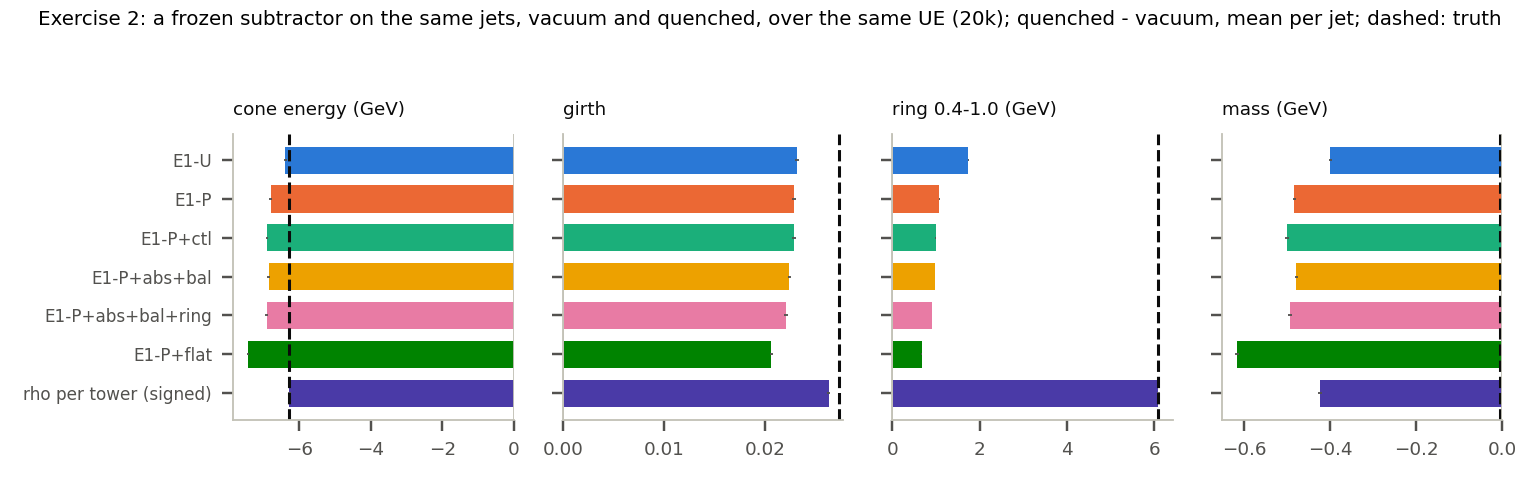
\includegraphics[width=\textwidth]{ex2_shifts.png}
\column{0.43\textwidth}
\scriptsize
\begin{itemize}\setlength\itemsep{0.15em}
\item \textbf{the recoil goes into the background}: 4.4-5.4 of the 6.1 GeV ring change ends in $\hat B$
  (Jamie: 98\%)
\item core change about right (102-118\%; Jamie 136\%), girth 75-85\% (69\%)
\item quenched cores lose more: 40\% of the hard-tower energy, 25\% in vacuum
\item no continuation of Exercise 1 changes it; the flat prior is the worst
\item the mass change ($-$0.4 GeV) appears for the standard readout too: not a clean observable here
\end{itemize}
\end{columns}
\end{frame}

% ---------------------------------------------------------------- 6
\begin{frame}{Exercise 3: clean translation. Population against correspondence}
\vspace{-0.3em}
\begin{center}
\tinytab{tables/ex3_population.tex}
\end{center}
\vspace{-0.3em}
\snote{20k held-out vacuum jets, one output each, against their true quenched versions; $W_1/\sigma$:
population distance (an independent quenched sample: 0.01-0.02). Shift recovered: 100\% = right.}
\vspace{0.1em}
\begin{columns}[T]
\column{0.52\textwidth}
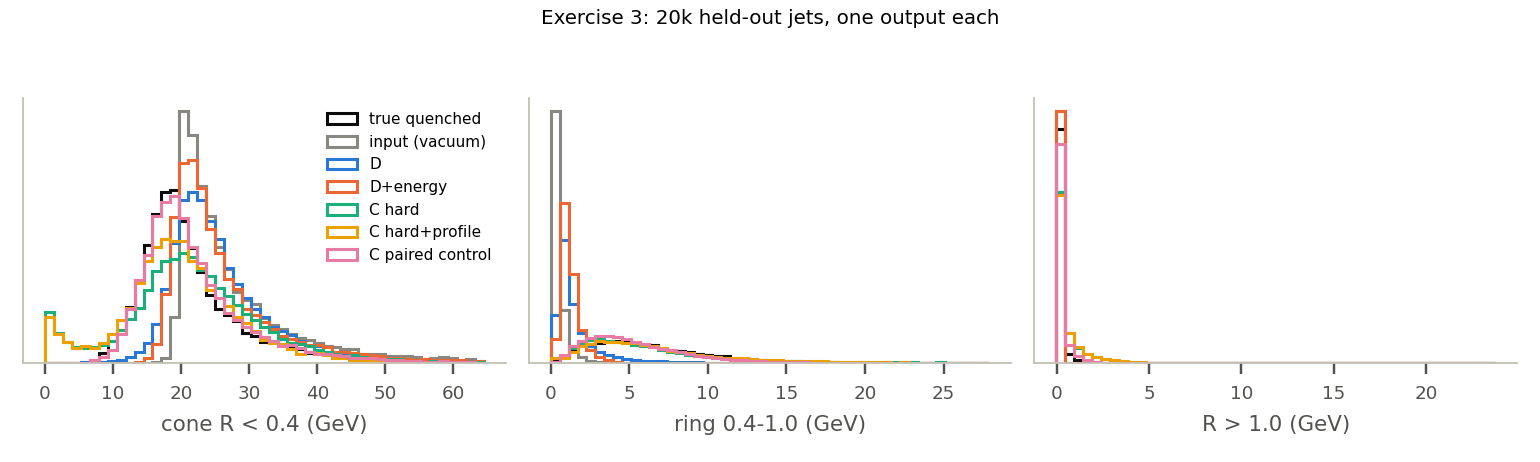
\includegraphics[height=0.3\textheight,width=\textwidth,keepaspectratio]{ex3_marginals.png}
\column{0.46\textwidth}
\scriptsize
\begin{itemize}\setlength\itemsep{0.1em}
\item \textbf{D} keeps each jet ($r$ 0.86) and quenches too little: 39-53\% of the core shift, 26-30\%
  of the ring. The energy term makes it change less (29\%, 14\%)
\item \textbf{C} \UP{} gets the population means (103-133\%) with real recoil towers, but ignores its
  input ($r$ 0.07) and places jets 0.13 off the axis (the spike at 0): the OT pairs' own offset
\item the \TP{} control: 95\%, 84\%, 85\%, tied to its input
\end{itemize}
\end{columns}
\end{frame}

% ---------------------------------------------------------------- 7
\begin{frame}{Exercise 3: the conditional law. Variation is not the right randomness}
\vspace{-0.3em}
\begin{center}
\tinytab{tables/ex3_conditional.tex}
\end{center}
\vspace{-0.3em}
\snote{100 test parents; 128 model draws each against 128 true quenchings (another 128: the true-vs-true
floor). Pre-registered: the law is recovered if $W_1 \le$ 1.5 $\times$ the paired control's and 68\%
coverage is 58-78\%.}
\vspace{0.1em}
\begin{columns}[T]
\column{0.55\textwidth}
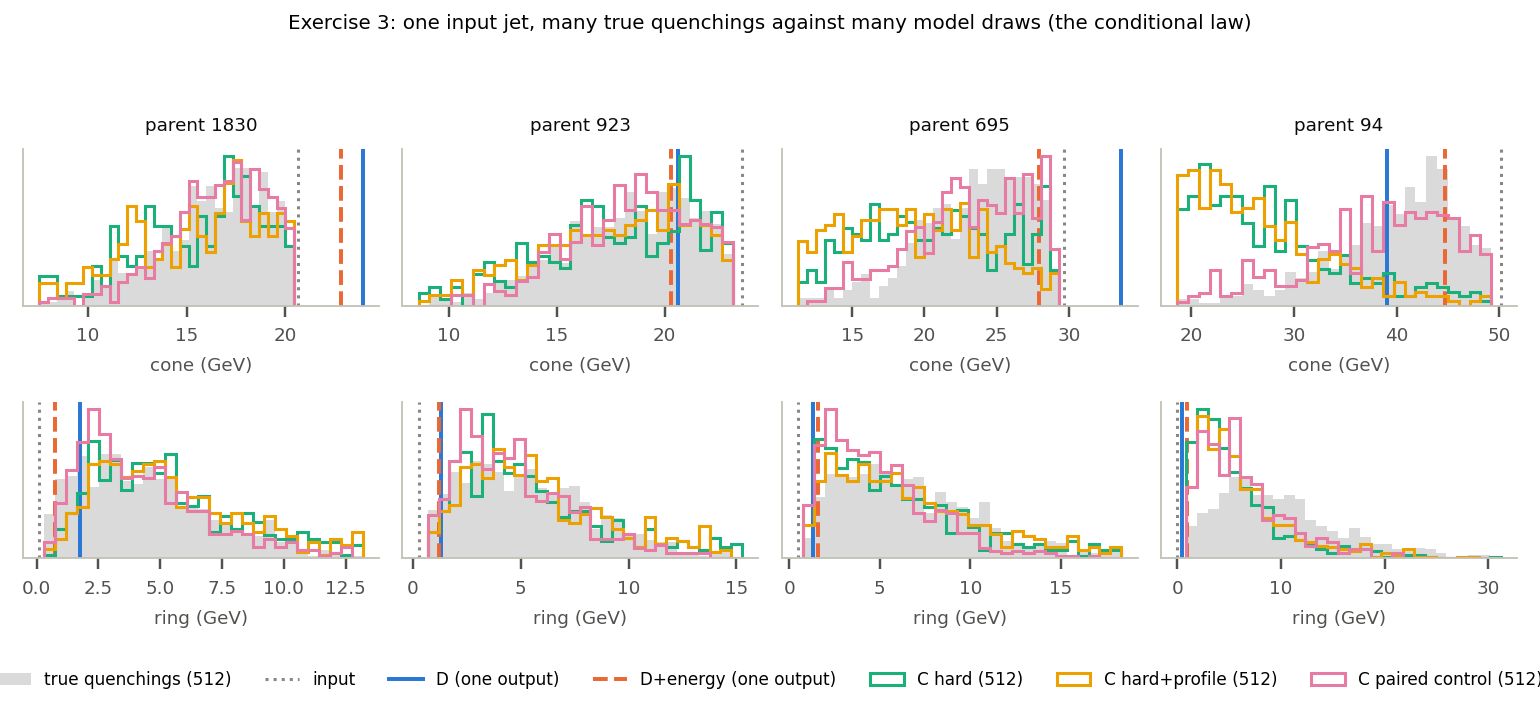
\includegraphics[height=0.34\textheight,width=\textwidth,keepaspectratio]{ex3_conditional.png}
\column{0.43\textwidth}
\scriptsize
\begin{itemize}\setlength\itemsep{0.1em}
\item \TP{}: the network can learn the toy's randomness (coverage 60-72\%, widths 0.9-1.1)
\item \UP{} C: a parent's draws spread like the whole population (cone sd 10-13 GeV against 3.8):
  variation, not the law. Profile and diversity terms change nothing
\item \textbf{girth rule}: the loss is predictable from the input (ceiling $r$ 0.97); C's follows the
  energy (+0.30), not the girth ($-$0.09), per jet $-$0.10. Jamie: +0.32, $-$0.12, $-$0.11
\end{itemize}
\end{columns}
\end{frame}

% ---------------------------------------------------------------- 8
\begin{frame}{Exercise 4: translate, and keep this event's UE}
\begin{columns}[T]
\column{0.57\textwidth}
\fittab{\linewidth}{tables/ex4_ue.tex}
\vspace{0.2em}
\snote{Input $J_\mathrm{vac} + B_a$, truth $J_\mathrm{med} + B_a$. Pre-registered: the event's UE is kept
if far towers correlate at $r \ge 0.99$ and change by $\le$ 10\% of the UE tower sd. Shifts with $\rho$
from the image's own $R > 1.2$; oracle: the true UE subtracted.}
\column{0.41\textwidth}
\scriptsize
\begin{itemize}\setlength\itemsep{0.1em}
\item whole-image OT pairs events by their UE: D spreads 6 GeV of the core over it ($r$ 0.989);
  penalties reach 0.995-0.996, at the 10\% line (0.095-0.108; the verdict flips with the seed)
\item \textbf{the near/far cost keeps the event's UE as the truth does} (0.9997) and recovers 114\% of
  the core change, 80\% of the ring (Jamie's best: 84\%, 69\%)
\item C regenerates the UE with every cost and penalty ($r$ 0.05-0.25): its spread is new UE
\end{itemize}
\end{columns}
\vspace{0.2em}
\begin{center}
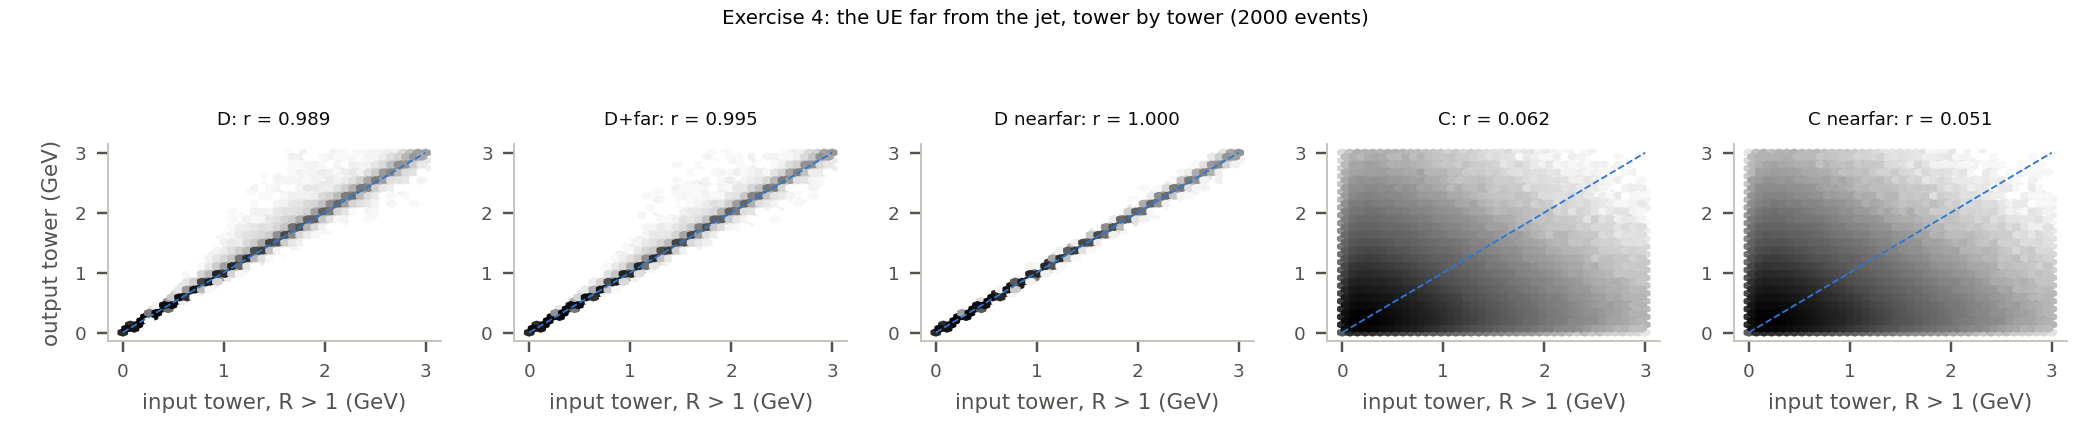
\includegraphics[height=0.21\textheight]{ex4_far.png}
\end{center}
\end{frame}

% ---------------------------------------------------------------- 9
\begin{frame}{Prior against data: the $2 \times 2$}
\begin{center}
\fittab{0.7\textwidth}{tables/prior_data.tex}
\end{center}
\vspace{-0.2em}
\snote{Each cell: 4000 updates from E1-P (a vacuum prior); \HY{}: synthetic sums from the cell's prior +
OT pairs of an independent mixture pool ($\lambda_U = 1$; both reach the gradient). Scored as Exercise 2;
bar chart: appendix A7.}
\vspace{0.3em}
\begin{columns}[T]
\column{0.55\textwidth}
\fittab{\linewidth}{tables/prior_data_effects.tex}
\column{0.43\textwidth}
\scriptsize
\begin{itemize}\setlength\itemsep{0.15em}
\item \textbf{the data matter} (beyond 3 sd): quenched data raise the recovered recoil 11\% $\to$
  30\%, girth 76\% $\to$ 90\% (vacuum prior). Jamie: identical to three digits
\item \textbf{not specifically}: they add ring to vacuum jets too; recoil $\le$ 30\%
\item \textbf{the prior invents recoil}: broad prior +0.5-0.7 GeV in vacuum jets (Jamie +0.7)
\item the UE-profile term breaks the subtraction ($-$3.9 GeV ring)
\end{itemize}
\end{columns}
\end{frame}

% ---------------------------------------------------------------- 10
\begin{frame}{A second seed, and an accurate solve}
\scriptsize
\textbf{Second seed} (the same inputs, both seeds; all \UP)

\vspace{0.2em}
\fittab{0.62\textwidth}{tables/seeds.tex}

\vspace{0.1em}
\snote{The best any deterministic predictor can reach with one true quenching's change: $r$ 0.48-0.50
(the bank's 256 quenchings per parent).}
\vspace{0.2em}
\begin{columns}[T]
\column{0.42\textwidth}
\scriptsize
\begin{itemize}\setlength\itemsep{0.15em}
\item Exercise 4: seeds agree jet by jet, neither predicts the jet's change; populations agree within
  2 points. \textbf{Agreement is not correctness} (Jamie: 0.84, 0.93; $-$0.02)
\item Exercise 3 D: population cone shift 39\% against 53\%
\end{itemize}
\column{0.56\textwidth}
\scriptsize
\textbf{Accurate solve}
\begin{itemize}\setlength\itemsep{0.15em}
\item all runs resolve at 32-256 NFE (validation) except the clean-jet D family and one penalty run
  at the 256 cap (1.6\%)
\item \textbf{E3-D does not converge}: starts $10^{-3}$ apart end 580$\times$ further apart, all from
  towers empty at both ends; 1-1.5 GeV per-jet noise at 256-1024 NFE
\item \textbf{a constraint learned through a coarse rollout holds for that rollout}:
\end{itemize}
\vspace{0.1em}
\fittab{0.78\linewidth}{tables/transfer.tex}
\end{columns}
\end{frame}

% ---------------------------------------------------------------- 11
\begin{frame}{Answers}
\footnotesize
\begin{enumerate}\setlength\itemsep{0.25em}
\item \textbf{Halo, core loss, lost recoil?} Core loss (25\%) and lost recoil (71-82\% into $\hat B$): yes;
  halo: no (2.1 GeV). Cause: the solve, not the regression. Losses change only the side effects
  (negative towers, halo $-$0.2 GeV, energy slope)
\item \textbf{Does a vacuum subtractor keep the medium modification?} The core change and most of the
  widening, not the recoil (18-29\%); quenched cores lose 40\%
\item \textbf{Conditional law or variation?} \UP{} C: variation with the right population, wrong law
  (output $r$ 0.07 with its input). \TP{} C: the law. The unpaired pairs, not the network, are missing
\item \textbf{This event's UE, or the population?} D with the near/far cost: this event's (as the
  truth). D with the whole-image cost: almost. C: the population only, whatever the penalty
\item \textbf{Do the mixture data matter beyond the prior?} Measurably (recoil 11\% $\to$ 30\%), unlike
  in Jamie's toy, but not specifically, and the prior still invents recoil
\item \textbf{What survives a second seed and an accurate solve?} Exercise 4's conclusions (both
  seeds, resolved solves); Exercises 1-2 and the C verdicts rest on resolved solves (one seed). Not the
  clean-jet D numbers (unresolved ODE, 14-point seed spread), and not constraints learned through coarse
  rollouts
\end{enumerate}
\vspace{0.4em}
\snote{Population agreement, event-preserving correspondence and the conditional law are reported
separately throughout. A success on this toy would justify a test on PYTHIA/JEWEL; it would not by
itself establish the physical modification.}
\end{frame}

% ---------------------------------------------------------------- 12
\begin{frame}{Limits, and what was not run}
\begin{columns}[T]
\column{0.5\textwidth}
\scriptsize
\textbf{Limits}
\begin{itemize}\setlength\itemsep{0.15em}
\item a reimplemented toy; unlisted details (grid, girth, UE redraws) are our choices
\item one seed except the two confirmations; 1.5 GPU hours per baseline, 4000-update continuations;
  the $2 \times 2$ are warm starts from one vacuum-prior checkpoint
\item the clean-jet D family is numerically unresolved; rollout terms trained through coarser solves than
  the test solve (except the last C arm)
\item matching costs: whole-image squared distance, and for Exercise 4 the one pre-specified near/far
  alternative (added for C after its whole-image run; disclosed)
\end{itemize}
\column{0.48\textwidth}
\scriptsize
\textbf{Not run}
\begin{itemize}\setlength\itemsep{0.15em}
\item PYTHIA jets in toy UE (Exercise 1 extension); our paired two-channel decomposer
\item C's diversity term in Exercise 4; a resampled-UE diagnostic
\item network widths, a compact backbone; longer training beyond the 4000-update controls
\item Jamie's discriminator, learning-rate and cycle-weight changes: no counterpart in OT-CFM
\end{itemize}
\vspace{0.4em}
\textbf{Next, if pursued}
\begin{itemize}\setlength\itemsep{0.15em}
\item a solve or path that keeps the subtractor's core (e.g.\ a noise-smoothed path, or reading out the
  one-step mean with a calibrated UE fluctuation)
\item a pairing that carries the jet's energy for C
\end{itemize}
\end{columns}
\end{frame}

% ================================================================ appendix
\appendix
\begin{frame}{A1. Coverage: Jamie's changes and their flow-matching counterparts (1/2)}
\tiny
\setlength{\tabcolsep}{2.5pt}
\begin{tabular}{p{0.2\linewidth}p{0.22\linewidth}p{0.22\linewidth}p{0.3\linewidth}}
\toprule
Jamie tried (printed slides) & his result & FM counterpart (runs) & our result \\
\midrule
GeV |error| per tower + balanced groups of jet, near-empty and far towers (Ex. 1) (51) & offset +9.9 -> +3.4 GeV; halo 9.6 -> 4.5 GeV & the same terms on the local endpoint surrogate (t <= 0.25), continuation of E1-P (E1-P\_absbal (B2) vs E1-P\_ctl (B1)) & no halo to fix (2.2 GeV); core loss unchanged (-24\%); negative towers 2.7\% -> 0.2\%; halo 2.2 -> 2.0 GeV. The terms act on the one-step surrogate, which is already right; the core is lost in the solve \\
+ ring energy sums (Ex. 1) (51-52) & offset +1.0 GeV, halo 3.4, scatter 2.6 GeV, fakes 0.3\% & + ring sums, same edges (surrogate) (E1-P\_absbalring (B3)) & no further change (core -24\%, halo 2.0 GeV, offset -5.3 GeV) \\
radial-profile rule, averaged over jets (Ex. 3) (90) & shift recovered core 95\%, ring 80\%, girth 36\% & batch-mean radial profile of C's solved outputs against an independent quenched batch (E3-Ch\_profile (B8) vs E3-Ch\_ctl (B7)) & population ring W1 0.21 -> 0.15, cone over-quenched (133\%); conditional law still wrong (cone W1 0.82); the term holds only partly at the test solve (x2.3) \\
total energy out = in (Ex. 3 v9) (85-87; 145) & stops the lazy solutions; core 89\%, ring 19\%, girth 32\%; energy 96\% +- 19\% per jet & total-GeV term on a differentiable 16-image midpoint rollout, continuation of E3-D (E3-D\_energy (B6) vs E3-D\_ctl (B5)) & pushes D toward changing less: core 39\% -> 29\%, ring 26\% -> 14\%, more haze; the toy itself keeps 99.72\% of the energy (exact equality is a prior) \\
dice: random numbers fed to the generator (Ex. 3 v10-v11, Ex. 4 v5) (91-92; 145-146) & samples 1/3 of the true spread (Ex. 3), then ignored with longer training; ignored (Ex. 4) & C: noise-driven conditional FM on the OT pseudo-joint, hard and entropic plans; true-paired control (E3-Ch, E3-Cs, E3-Cp; E3g-C; E4-C) & C makes real variation but not the conditional law: a parent's spread is the population's (cone sd 11.6 vs 3.8 GeV), output r 0.07 with the input; the true-paired control recovers the law (coverage 60-72\%) \\
diversity rule: different dice, different output (Ex. 3 v12, Ex. 4 v6) (92; 145-146) & spread a free knob: 1.6 vs 4.7 GeV (Ex. 3), 8.0 vs 4.5 GeV (Ex. 4) & capped mode-seeking term between two solved C draws (cap from target pairs) (E3-Ch\_div (B9); Ex. 4: not run (budget)) & changes nothing (C already too diverse; cone W1 0.88); Ex. 4 not run \\
no identity rule (Ex. 4 v1) (98; 146) & half the ring, core overshot, UE inverted (far-tower r -0.52) & D without any invariance term; its unchanged continuation (E4-D (A9), E4-D\_ctl (B10)) & D keeps the UE nearly (far r 0.989, no inversion) but spreads 6 GeV of the core over it; C regenerates the UE (r 0.06) \\
identity rule everywhere (Ex. 4 v2) (99; 146) & near-copy: UE kept, no ring & global output-change penalty on solved endpoints (E4-D\_global (B11)) & far r 0.995, rms 0.108 (still above the 10\% limit); suppresses the quenching (ring 15\%) \\
identity rule only at R > 1.0, + energy conservation (Ex. 4 v3-v5) (99-100; 146) & near-copy at first (core 30\%, no ring); after 4x training core 78-84\%, ring 65-70\%, UE unchanged & output-change penalty at R >= 1.0 on solved endpoints; also with the near/far matching cost and for C (E4-D\_far (B12), E4-Dnf\_far (B13), E4-C\_far (B15)) & D: far r 0.995, ring 26\% (full cost); with the near/far cost 0.9999, core 108\%, ring 68\%; C: far r 0.25 (8-NFE rollout, holds only at 8 NFE) and 0.07 (accurate rollout) \\
jets below the 20 GeV training range; jets flat in 5-80 GeV (Ex. 1, v7) (54; 145) & -6 GeV at 5-10 GeV: bent toward known jets; flat 5-80 GeV: better above 60 GeV, 5-15 GeV still poor & 5-20, 60-80, 80-100 GeV test slices; flat 5-80 GeV prior continuation (E1-U, E1-P; E1-P\_flat (B4)) & slices: -3.1/-9.6/-10.8 GeV (E1-U at 5-20/60-80/80-100); flat prior: slope 0.94 -> 0.98, 60-80 GeV -6.9 -> -5.7 GeV, 5-20 GeV worse (-4.0), core loss unchanged \\
\bottomrule
\end{tabular}

\end{frame}

\begin{frame}{A1. Coverage (2/2)}
\tiny
\setlength{\tabcolsep}{2.5pt}
\begin{tabular}{p{0.2\linewidth}p{0.22\linewidth}p{0.22\linewidth}p{0.3\linewidth}}
\toprule
Jamie tried (printed slides) & his result & FM counterpart (runs) & our result \\
\midrule
longer training (Ex. 1 v8: x4; Ex. 3 v11: x4, +2400 steps; Ex. 4 v4: x4) (50-51; 90; 145-146) & Ex. 1 offset +13 -> +11 GeV; Ex. 3 core 78\% -> 155\%; Ex. 4 near-copy -> core 78\%, ring 65\% & unchanged-loss continuations of 4000 updates; validation curves (E1-P\_ctl, E3-D\_ctl, E3-Ch\_ctl, E4-D\_ctl) & +4000 updates: Ex. 1 unchanged; Ex. 3 D cone 39\% -> 52\%; C, Ex. 4 D unchanged \\
two trainings, different random start (Ex. 4 v4s2) (101; 146) & agree jet by jet (r 0.84, 0.93), not with the truth (-0.02) & seed 1 of E4-D (+ far penalty) and of E3-D; same inputs' outputs compared (E4-D\_s1 (A13), E4-D\_s1\_far (B14), E3-D\_s1 (A12)) & Ex. 4: seeds agree jet by jet (r 0.85, 0.90), each 0.08-0.10 with the true change (ceiling 0.48); Ex. 3: seeds r 0.65/0.81, population cone shift 39\% vs 53\% \\
loss set by the jet's girth (Ex. 3 toy variant) (109) & losses follow energy (+0.32) not width (-0.12); per jet vs truth -0.11 & D and C trained on separate girth-rule pools (E3g-D (A7); E3g-C (A8)) & D: loss follows girth 0.22, energy 0.15, true loss 0.17; C: girth -0.09, energy +0.30, true loss -0.10 (ceiling 0.97) \\
vacuum or broad prior x vacuum or quenched data (Ex. 1 setup) (116-119) & vacuum prior: girth +0.019/+0.020, ring +0.2/+0.2 of +5.7 GeV either data; broad: girth +0.023, ring +0.9 in vacuum jets & hybrid L\_syn + L\_unp (lambda\_U = 1), four cells and two synthetic-only arms, continuations of E1-P (PD\_vac\_vac, PD\_vac\_q, PD\_broad\_vac, PD\_broad\_q (B16-B19); PD\_vac\_syn, PD\_broad\_syn (B20-B21)) & data matter (ring +1.18 GeV, 72 sd, vacuum prior) but recoil <= 30\% and quenched data add ring to vacuum jets too; broad prior +0.5-0.7 GeV ring in vacuum jets \\
batch-averaged UE around the jet must be flat (Ex. 1 setup) (122-123) & girth 61\% -> 70\%, recoil 0.3 of 5.7 GeV, +2.8 GeV ring in vacuum jets & batch-mean UE radial profile of B\_hat against independent UE under the same geometry, on the vacuum-prior x quenched-data cell (PD\_vac\_q\_ueprof (B22)) & breaks the subtraction: vacuum-jet ring -3.9 GeV, quenched ring change -24\%, 29\% of quenched jets lost \\
vacuum-trained subtractor on quenched jets (Ex. 2) (70-76) & cone 136\%, girth 69\%, ring 2\%, mass -0.7 GeV invented, 12\% of quenched jets lost & the frozen Exercise 1 checkpoints on held-out pairs with shared UE (E1-U, E1-P and the E1-P continuations) & cone 102-108\%, girth 85\%, ring 18-29\% (recoil 4.4-5.0 GeV in B\_hat), mass -0.4 GeV (as for rho readouts), 14-15\% of quenched jets below 10 GeV; continuations change none of it \\
0.2M -> 0.9M -> 3.5M parameters (Ex. 1) (50) & offset +13.4 -> +8.6 GeV & not run: one fixed backbone (UVCGAN-S ViT-ModNet, 32M); no architecture search & - \\
identity term and cycle weight 100; whole-image discriminator heads, three discriminators, cycle weight 10 -> 2 and discriminator learning rate x2 (48; 57-60; 145) & identity + cycle 100: halo worse & not applicable: OT-CFM has no discriminator, cycle or identity loss & - \\
PYTHIA jets in toy UE (Ex. 1) (55-56) & the same halo and the same cure & deferred (budget) & - \\
- (-) & - & our paired two-channel decomposer on the toy: optional, not run & - \\
\bottomrule
\end{tabular}

\end{frame}

\begin{frame}{A2. Run ledger (training time on A6000s; 32.4 GPU hours in all)}
\begin{columns}[T]
\column{0.49\textwidth}
\fittab{\linewidth}{tables/ledger_a.tex}
\column{0.49\textwidth}
\fittab{\linewidth}{tables/ledger_b.tex}
\end{columns}
\vspace{0.3em}
\snote{From: the base of a continuation (4000 updates); NFE: the frozen midpoint solve of the scored
outputs. E3-D\_energy, E3-Ch\_div, E4-Cnf\_far: the rollout terms make their updates slower.}
\end{frame}

\begin{frame}{A3. Solver: the frozen accuracy of every baseline}
\begin{center}
\scriptsize
\setlength{\tabcolsep}{3pt}
\begin{tabular}{lrlrrrrr}
\toprule
 & frozen & & \multicolumn{3}{c}{$N$ against $2N$ (validation)} & \multicolumn{2}{c}{4 Euler steps} \\
run & NFE & resolved & key / change & $W_1$ shifts & key / two noises & key / change & ms / image \\
\midrule
E1-U\_s0 & 32 & yes & 0.001 & within sd & -- & 0.17 & 1.1 / 8.7 \\
E1-P\_s0 & 32 & yes & 0.001 & within sd & -- & 0.04 & 1.1 / 8.7 \\
E3-D\_s0 & 256 & no & 0.256 & beyond sd & -- & 3.16 & 1.1 / 70.1 \\
E3-Ch\_s0 & 64 & yes & 0.009 & within sd & 0.009 & -- & -- \\
E3-Cs\_s0 & 128 & yes & 0.004 & within sd & 0.004 & -- & -- \\
E3-Cp\_s0 & 64 & yes & 0.006 & within sd & 0.008 & 0.45 & 1.1 / 17.6 \\
E3g-C\_s0 & 128 & yes & 0.003 & within sd & 0.002 & -- & -- \\
E4-D\_s0 & 64 & yes & 0.005 & within sd & -- & 1.19 & 1.1 / 17.6 \\
E4-D\_s1 & 64 & yes & 0.009 & within sd & -- & -- & -- \\
E4-Dnf\_s0 & 64 & yes & 0.003 & within sd & -- & -- & -- \\
E4-C\_s0 & 32 & yes & 0.001 & within sd & 0.003 & -- & -- \\
\bottomrule
\end{tabular}

\end{center}
\snote{N against 2N on 1000 validation inputs (for C the same noise): adequate when the key per-image
energy moves by less than 1\% of the model's change, every $W_1$ shift stays within its bootstrap sd, and
for C the change is below 1/10 of that between two noises; otherwise N doubles, to 256 at most. Four Euler
steps: a speed diagnostic only. Continuations: checked at their base's N and re-solved by the same rule
when they fail.}
\end{frame}

\begin{frame}{A4. Exercise 1: fixed held-out events}
\begin{center}
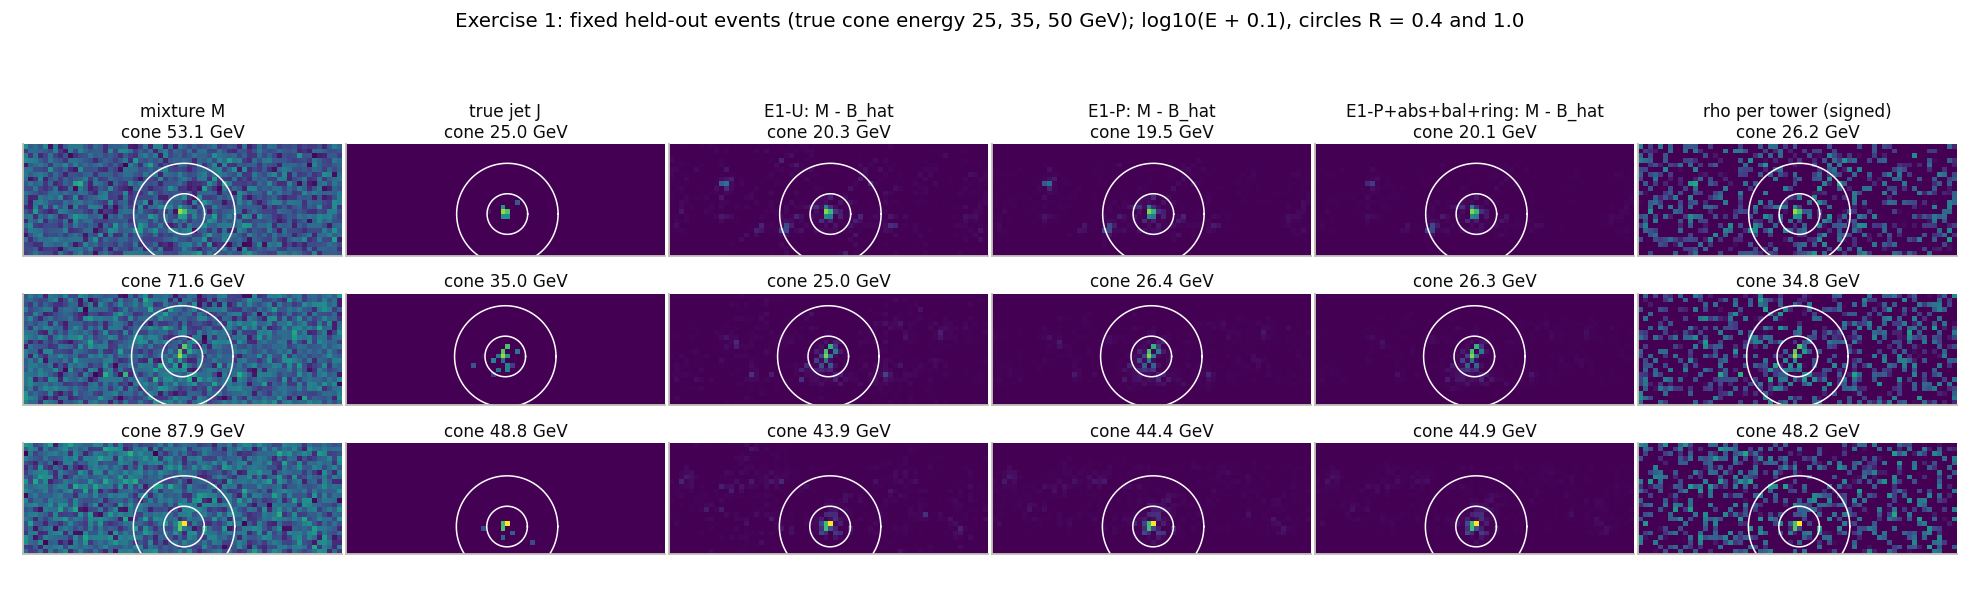
\includegraphics[width=\textwidth]{ex1_displays.png}
\end{center}
\end{frame}

\begin{frame}{A5. Exercise 3: one parent, true quenchings and model draws}
\begin{center}
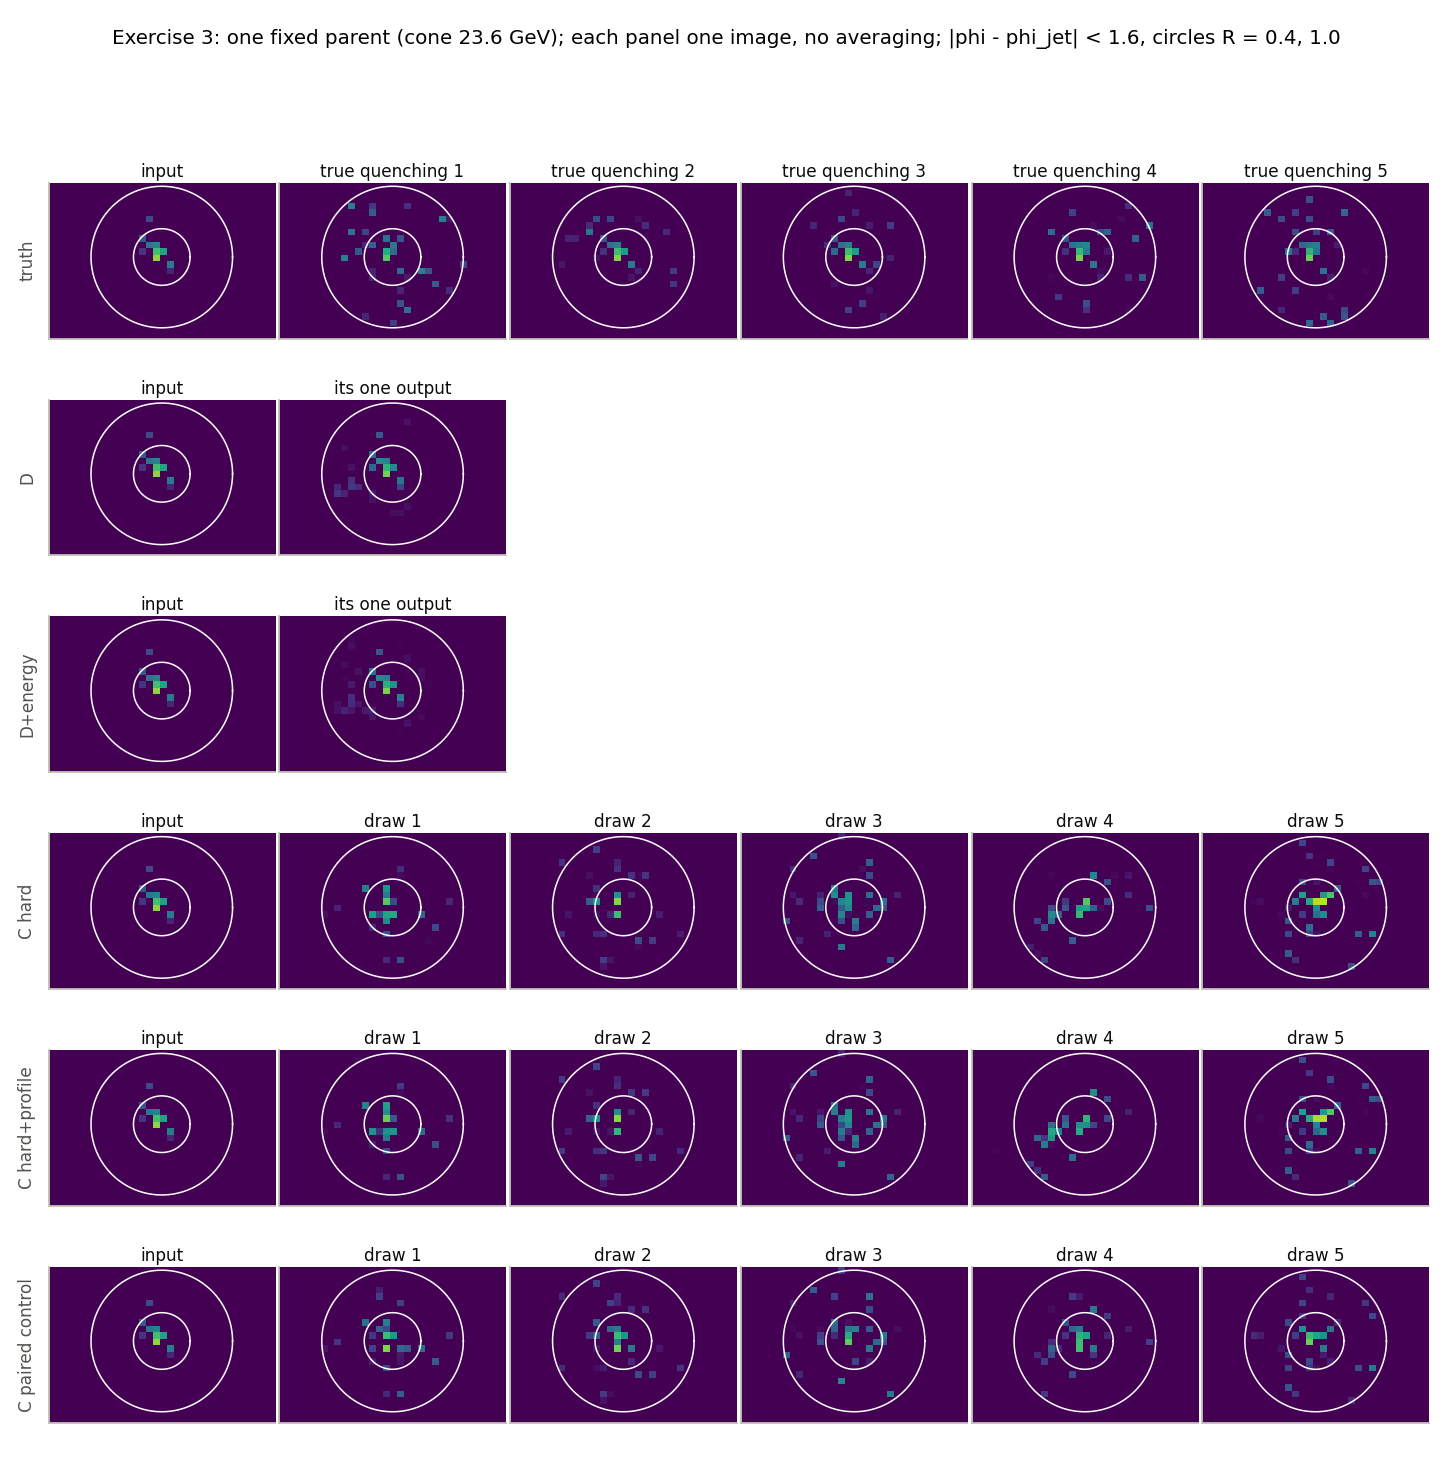
\includegraphics[height=0.82\textheight]{ex3_displays.png}
\end{center}
\end{frame}

\begin{frame}{A6. Exercise 4: one parent, true quenchings and model draws}
\begin{center}
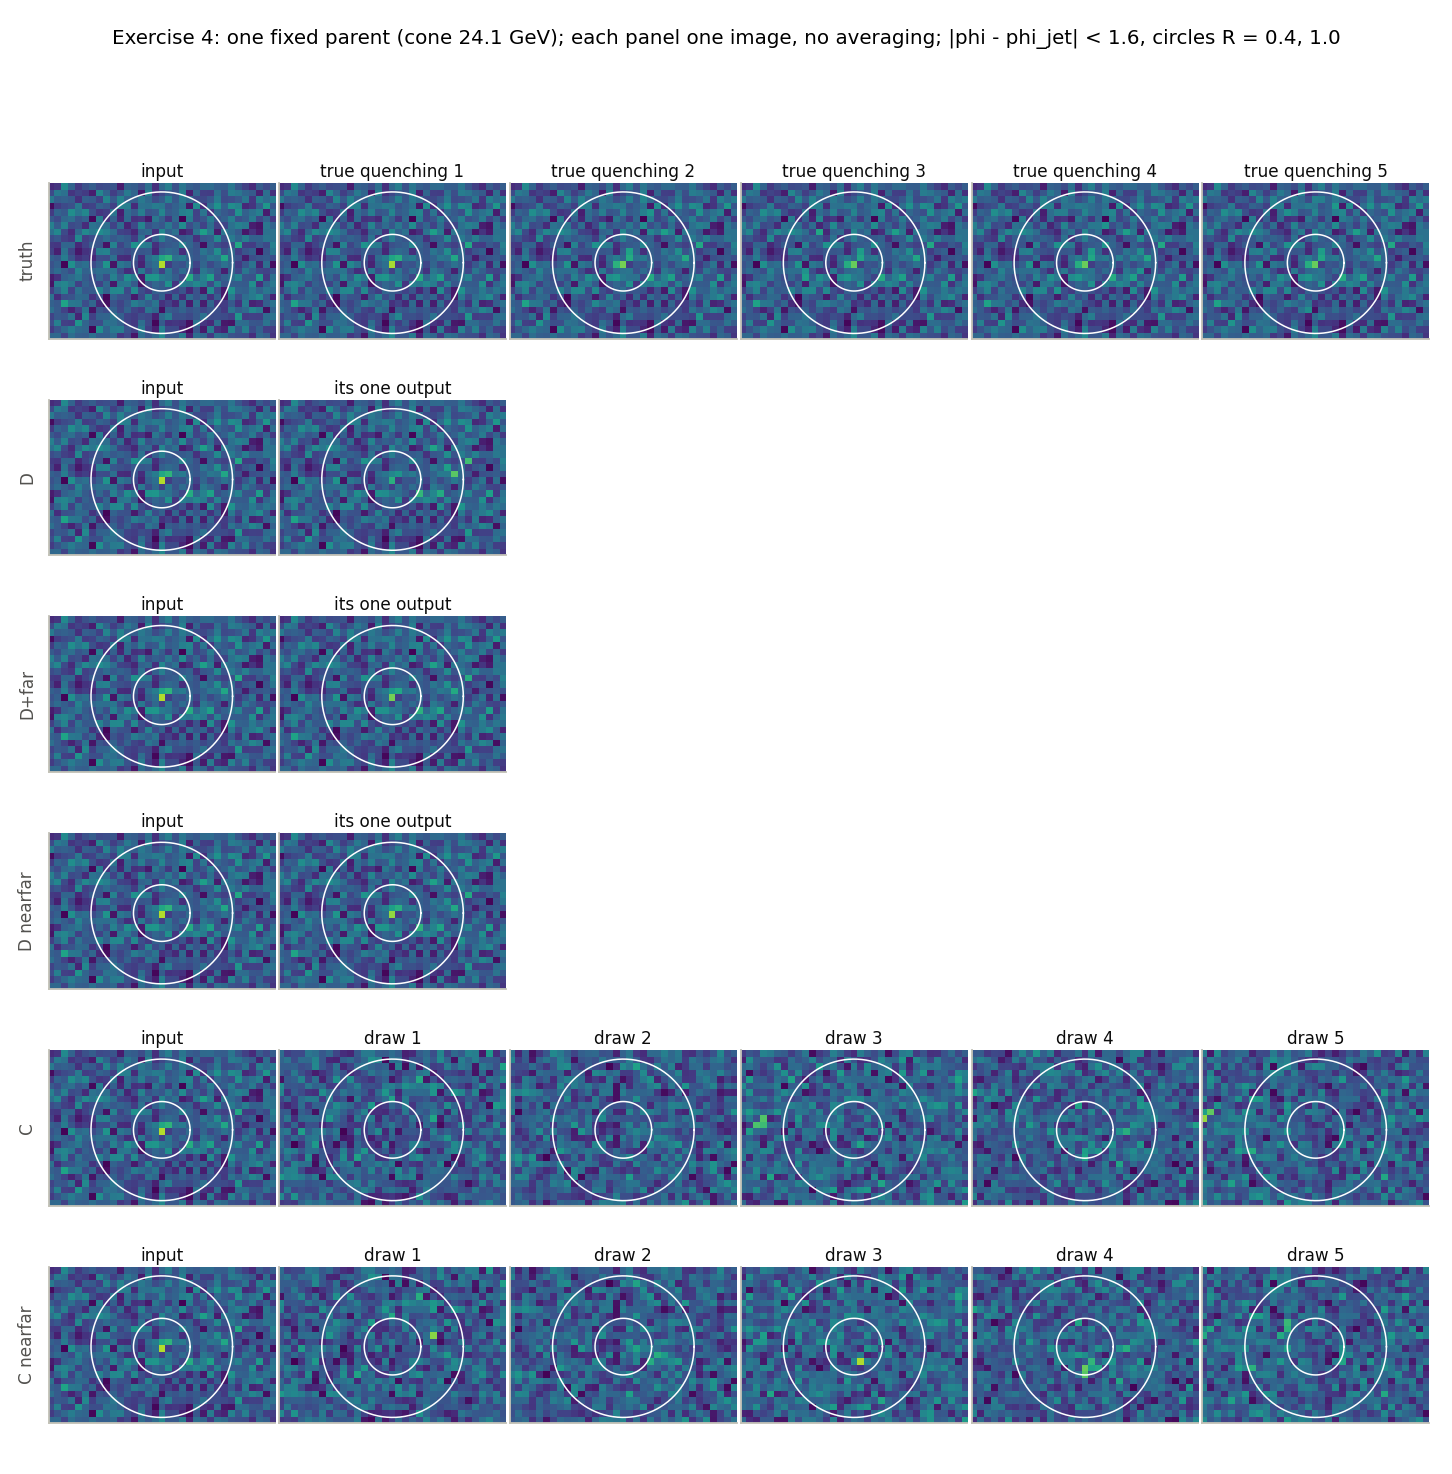
\includegraphics[height=0.82\textheight]{ex4_displays.png}
\end{center}
\end{frame}

\begin{frame}{A7. Prior against data: the shifts of every cell}
\begin{center}
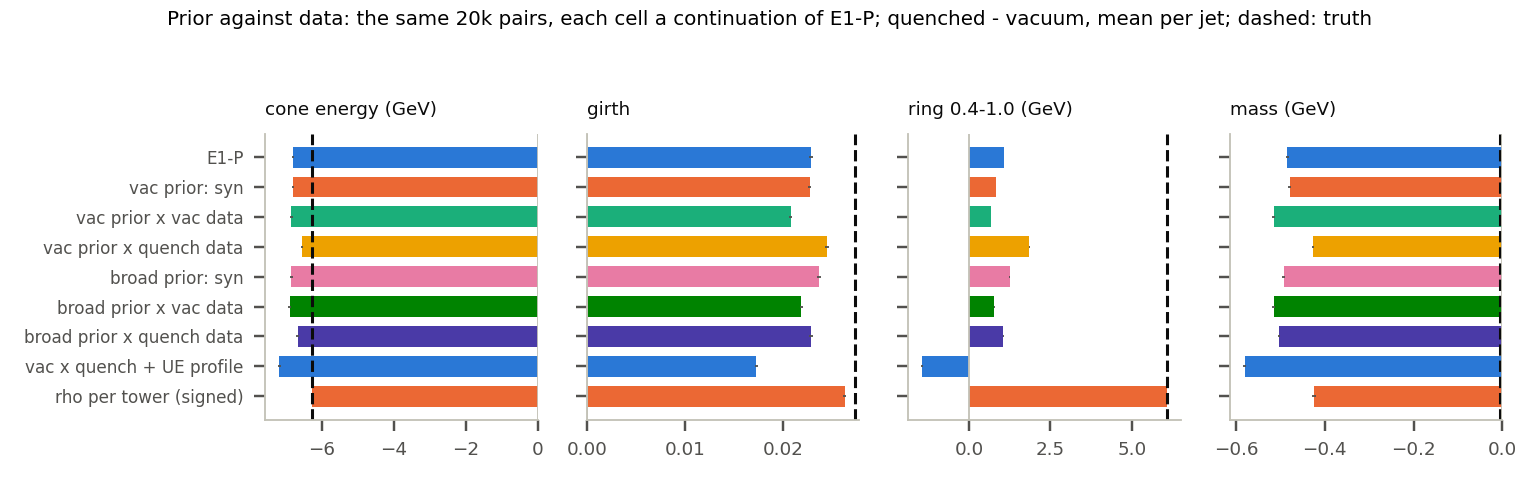
\includegraphics[width=\textwidth]{prior_data_shifts.png}
\end{center}
\end{frame}

\end{document}
